\documentclass[UTF8]{ctexart}


\usepackage{amsmath}
\usepackage{graphicx}
\usepackage{authblk}


\setCJKmainfont{Source Han Sans CN}

\setmainfont{Times New Roman}

\pagestyle{empty}

\newcommand{\mat}[1]{\begin{bmatrix} #1 \end{bmatrix}}

\title{从几何意义认识线性代数}
\author[*]{XXX}
\affil[*]{XXXX}
\date{2024.6}
\begin{document}
\maketitle
\section*{引言}

在完成了学校安排的线代课程后,我掌握了许多关于矩阵,行列式与线性方程组的计算,比如算行列式,算特征值,特征向量,算矩阵乘积,但是却不理解为什么矩阵的乘法这样定义,不了解行列式到底是什么 —— 我只知其然而不知其所以然。一些对于线性代数的意义的理解是必要的。本文是~\cite{Essenceoflinearalgebra}~\cite{linearalgebraforeveryone}后的笔记与总结。以期能高屋建瓴,对线性代数有更加深刻的认识。

\pagebreak

\tableofcontents

\pagebreak

\section{线代基础概念}

\subsection{向量与线性组合}

要讨论矩阵,首先应讨论向量。高中数学中已经确定了向量的几何意义 —— 即向量是使用数组描述的,从原点出发,指向由数组确定的终点坐标的,带有方向与长度的线段。由此,我们可以定义向量的加法与向量的乘法。

\begin{figure}[hb]
    \centering
    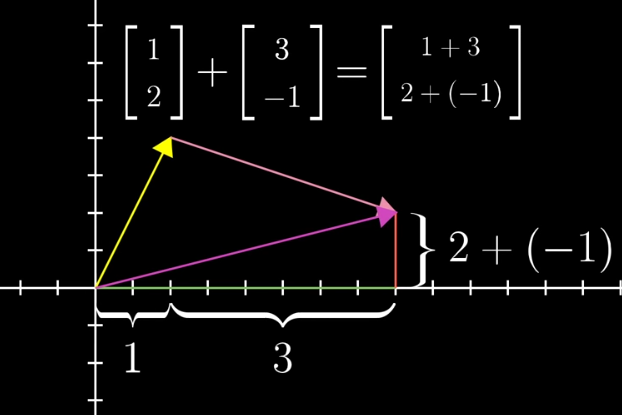
\includegraphics[width=0.7\textwidth]{./figs/vector_add.png}
    \caption{向量的加法}
    \label{fig:vector_add}
\end{figure}

如公式~\ref{fig:vector_add}所示,向量的加法既可以在几何视角上认为是从起点按照加数给出的确定的向量走到终点也就是和向量的过程,也可以在数学意义上认为是两个向量对应位置相加的结果。据此,可以给出向量乘法的定义:在几何意义上,向量的乘法可以认为是向量沿其方向拉伸,对于负数,则是将向量沿其方向压缩。数学家们使用标量(scalars)描述拉伸,压缩的程度。即向量乘法可以看成原坐标中的各个值按照对应的标量缩放(与标量相乘)。

更进一步地,通过引入空间的\textbf{基向量}的概念,如公式~\ref{eq:vectorbase}所示,向量可以被表示为基向量$\hat{i}, \hat{j}$的与标量相乘后的和(线性组合)。基向量的定义: 基向量是向量空间里某一群特殊的向量,使得向量空间中的任意向量,都可以唯一地表示成基向量的线性组合(或线性组合的极限)。

\begin{equation}
    \label{eq:vectorbase}
    \begin{bmatrix}
        3 \\ -2
    \end{bmatrix} = 3\hat{i} + -2\hat{j}
\end{equation}

所有可以表示为给定向量线性组合的向量的集合被称为给定向量张成的空间,而给定的向量则被称为空间的基向量。引入线性相关的概念,当多个向量取其一而不减小张成的空间的维度,则称这组向量是线性相关的,反之,则称这组向量是线性无关的。

\subsection{矩阵与行列式}

\subsubsection{线性变换}
要解释矩阵,首先要明确变换的概念。从直觉出发,变换可以被看成一个函数,它以一个向量作为输入,并输出另一个向量。~\cite{Essenceoflinearalgebra}中指出变换之所谓被称为变换而非函数,是为了暗示\textbf{运动}的观点 —— 向量的终点从输入运动到输出(前面提到过向量是以原点为起点的),如图~\ref*{fig:vector_transform}。

\begin{figure}[hb]
    \centering
    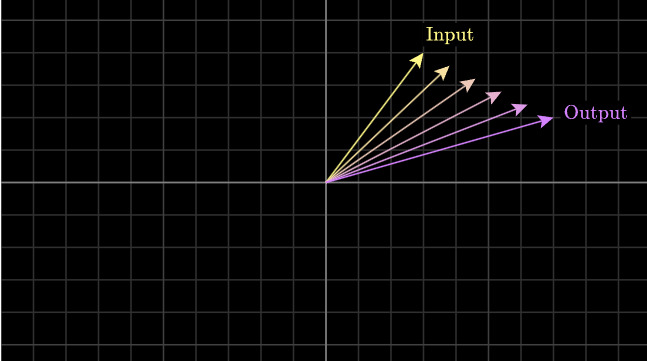
\includegraphics[width=0.7\textwidth]{./figs/vector_transform.png}
    \caption{向量变换}
    \label{fig:vector_transform}
\end{figure}

为了更直观的展示变换的形状,可以在无限网格上变换所有点。如图~\ref*{fig:grid_transform}

\begin{figure}[hb]
    \centering
    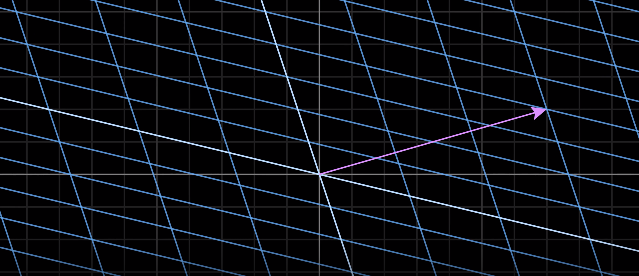
\includegraphics[width=0.7\textwidth]{./figs/grid_transform.png}
    \caption{向量变换}
    \label{fig:grid_transform}
\end{figure}

线性变换的概念可以通过图~\ref{fig:linear_transform}快速且直观的给出。线性变换是(对于网格体系而言)保持网格线平行等距且网格原点位置不变的变换。

\begin{figure}[hb]
    \centering
    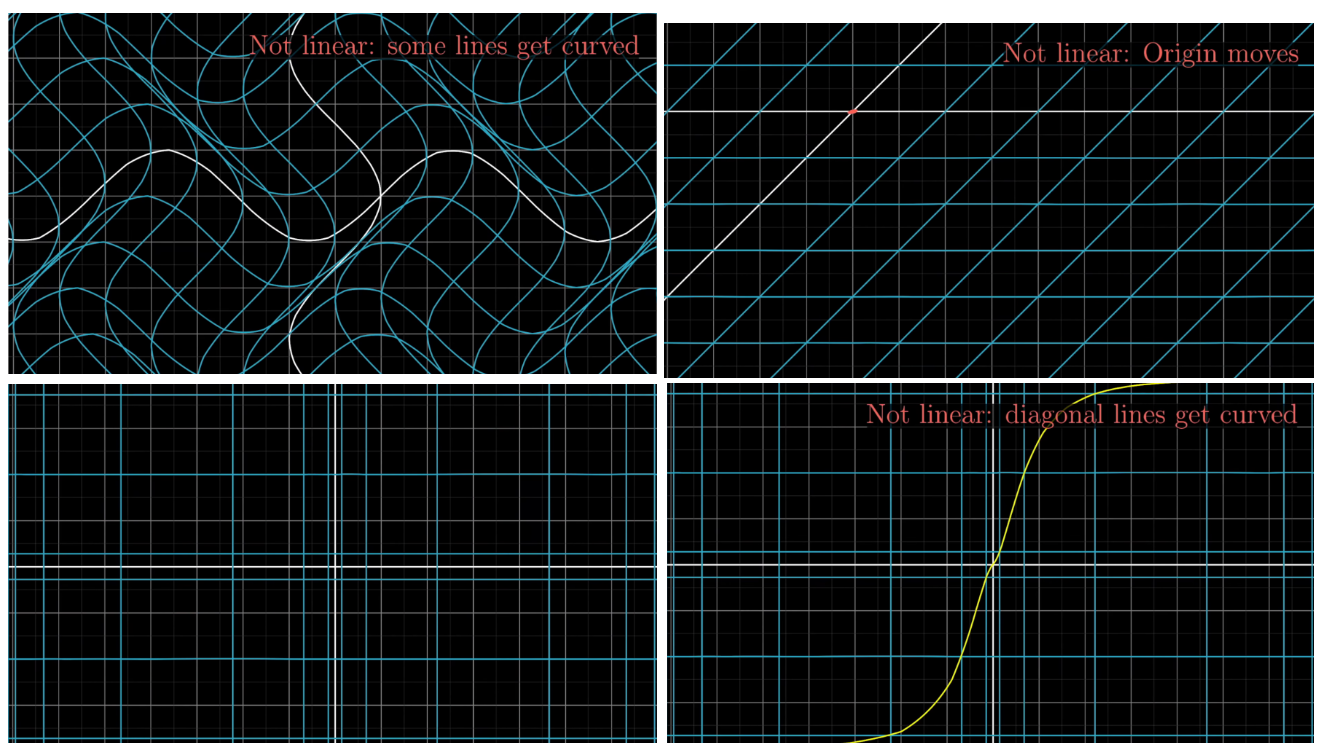
\includegraphics[width=0.7\textwidth]{./figs/linear_transformation.png}
    \caption{非线性的变换}
    \label{fig:linear_transform}
\end{figure}

\subsubsection{矩阵与矩阵乘法}
我们已经拥有了线性变换的概念,此时我们需要使用某种记法来描述一个线性变换。结合前面提到的基向量与变换无限平面的思想,可以很快的得出一个线性变换的记法 —— 记录空间的基向量。比如说对于二维空间而言,记录$\hat{i}$与$\hat{j}$,原向量与新的基向量相乘即可得到新的基向量下对应的新向量 —— 即原向量经过线性变换后的结果。

\begin{align*}
    vector &= \begin{bmatrix} -3 \\ -1 \end{bmatrix}, \hat{i} = \begin{bmatrix} -1 \\ 1\end{bmatrix}, \hat{j} = \begin{bmatrix} -2 \\ -1\end{bmatrix} \\
    L(\vec{v}) &= -3\begin{bmatrix} -1 \\ 1\end{bmatrix} - 1\begin{bmatrix} -2 \\ -1\end{bmatrix} \\
    &= \begin{bmatrix} -3(-1) - 1(-2) \\ -3(1)-1(-1) \end{bmatrix} \\
    &= \begin{bmatrix}
        5 \\ -2
    \end{bmatrix}
\end{align*}

这时我们可以粗糙的定义一个矩阵-向量乘法的概念:将矩阵放在向量的左边,让矩阵像函数一样,向量则是函数的输入变量。

延申的,我们可以得到矩阵-矩阵乘法的意义,先应用一个线性变换,再应用一个 —— 组合变换(将它们的效果综合)起来成为一个新的矩阵,这就是矩阵-矩阵乘法。

\begin{figure}[hb]
    \centering
    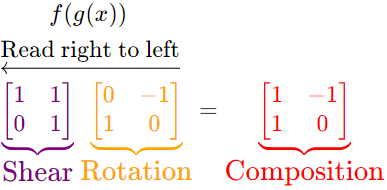
\includegraphics[width=0.7\textwidth]{./figs/m_multication.png}
    \caption{从函数角度考虑矩阵乘法}
    \label{fig:m_multication}
\end{figure}

矩阵与矩阵的乘法可以从矩阵分解~\cite{Artoflinearalgebra}的角度出发,给出四个视角图~\ref{fig:4_vies_m_multication}

\begin{figure}[hb]
    \centering
    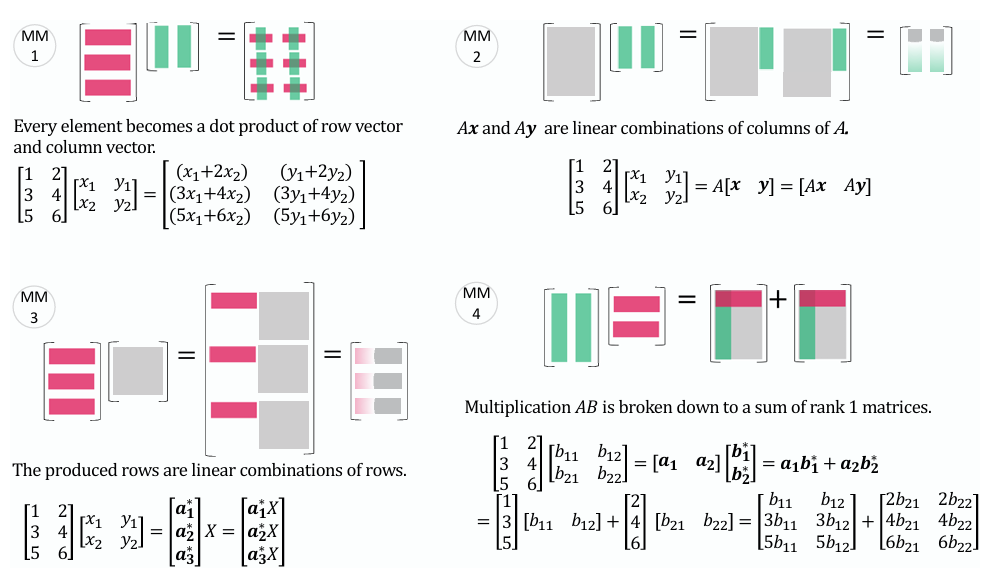
\includegraphics[width=0.7\textwidth]{./figs/4sight_m_multication.png}
    \caption{矩阵-矩阵乘法的四种分解视角}
    \label{fig:4_vies_m_multication}
\end{figure}

\subsubsection{行列式}

行列式用于估计线性变换改变面积的比例(由于网格线平行等距,对任意图形缩放比例相等)

\begin{figure}[hb]
    \centering
    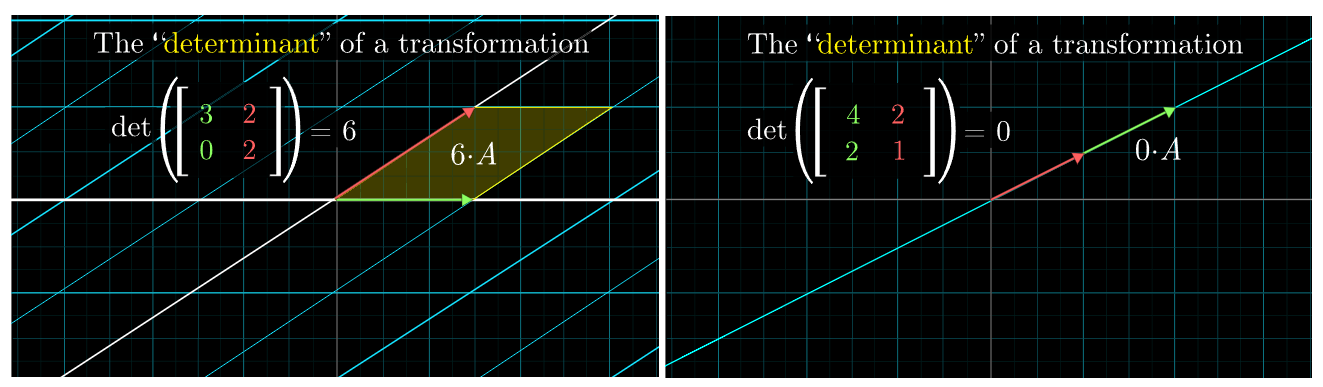
\includegraphics[width=0.7\textwidth]{./figs/det_special.png}
    \caption{行列式的特殊情况}
    \label{fig:det_special}
\end{figure}

图~\ref{fig:det_special}从集合角度展示了:1. 左图展示了为什么上/下三角行列式的值为对角线的乘积 —— 这种矩阵是\textbf{shear}变换(正方形的格子变为平行四边形),因为求取面积的公式不变,仍是长乘以宽。2. 右图展示了为什么成倍数的行会使行列式的值为0 —— 这涉及到线性相关的概念(当A与B线性相关,证明B的加入并未展出新的空间),当考虑2维的情况,这个矩阵是一条线,在二维空间里一条线的面积为0,因此具有线性相关行的行列式的值为0。

\subsubsection{逆变换}
对于线性方程组,可以将其转换为$A\vec{x}=\vec{v}$的形式,其中$A$是系数矩阵,$\vec{x}$是未知数的向量,$\vec{v}$是常数向量。从几何角度看,$\vec{x}$与$A$相乘后得到$\vec{v}$ —— $\vec{x}$通过线性变换$A$变换为$\vec{v}$。于是,为了找到$\vec{x}$,我们需要一种逆变换$A^{-1}$将$\vec{v}$移回$\vec{x}$。

\textbf{$A^{-1}$抵消了$A$带来的变换},那么下面的公式就可以很容易的得出 —— 没有变换所以仍是空间最初始的基向量

\begin{equation}
    A^{-1}A = \begin{bmatrix}1 & 0 \\ 0 & 1\end{bmatrix}
\end{equation}

由此出发可以讨论矩阵行列式为0的情况 —— 矩阵的维度被压缩。从直觉出发,det为0的矩阵是无解的 —— 从一个点映射到一条线是不可能的。只有一种例外的情况,求解的向量$\vec{x}$刚好落在这条线上。

\subsubsection{列空间与秩}
更进一步的我们将讨论列空间与秩。列空间就是矩阵的列所张成的空间。这句话可能难以理解,但是很好解释 —— 矩阵的列是矩阵的基向量,基向量的展开(与任意向量相乘)则可以得到这个矩阵所有的可能输出。此时可以给出秩的定义:秩是列空间的维数,代表着变换后空间的维数,其最大值为矩阵的列数,达到最大值时称为\textbf{矩阵满秩}。

矩阵的零空间是变换后落在原点的向量的集合,由其定义,三个性质易得: 1. 零空间始终包含在列空间中(线性变换要求原点不变);2. 对于满秩矩阵(变换),零空间是唯一的。3. 对于非满秩矩阵(变换),零空间不唯一。

非方阵的几何意义:改变维度。下面公式所示的矩阵是从二维到三维的映射。

\begin{align*}
    \begin{bmatrix}
        -2 &0 \\ -1 & 1\\ -2 & 1
    \end{bmatrix} \\
    \hat{i} = (-2,-1,-2) \\
    \hat{j} = (0,1,1)
\end{align*}

\subsubsection{向量点积}
向量的点积$v\cdot w$是从几何上可以看作$w$在$v$方向上的投影的\textbf{长度}与$v$长度的乘积。对于结果的正负可以很容易给出:
\begin{itemize}
    \item $v\cdot w > 0$ $v$,$w$夹角小于90度(近似同向)
    \item $v\cdot w = 0$ $v$,$w$相互垂直。
    \item $v\cdot w < 0$ $v$,$w$夹角大于90度(反向)
\end{itemize}

点积的结果与点积的顺序无关:对于相同长度的两向量的点积可以容易的通过对称性证得,而在不同长度的两向量的点积失去对称性,但是结论依旧是相同的。

点积与投影的关系:对偶性。在~\cite{Essenceoflinearalgebra}中花了较大篇幅进行讨论,由于本文篇幅有限,仅作简单的推导论述:如公式~\ref{eq:projection_dot},$\begin{bmatrix}1 & -2\end{bmatrix}$为变换,$\begin{bmatrix}4 \\3\end{bmatrix}$为向量。设数轴一个单位向量为$\hat{u}$,$\hat{i}$对$\hat{u}$所在直线的投影与$\hat{u}$向$x$轴的投影完全对称,$\hat{j}$同理,因此可以得出结论二维空间向该数轴的线性变换为$\begin{bmatrix}u_x & u_y\end{bmatrix}$,可以得到公式~\eqref{eq:m_v_production}(矩阵与向量的乘积) ,\eqref{eq:v_v_dot} (点积)

\begin{equation}
    \label{eq:projection_dot}
    \begin{bmatrix}1 & -2\end{bmatrix}\begin{bmatrix}4 \\3\end{bmatrix} = 4 \cdot 1 + 3 \cdot (-2)
\end{equation}

\begin{align}
    \mat{u_x & u_y}\mat{x\\y} &= u_x \cdot x + u_y \cdot y \label{eq:m_v_production} \\
    \mat{u_x & u_y}\mat{x\\y}\mat{x\\y} &= u_x \cdot x + u_y \cdot y  \label{eq:v_v_dot} 
\end{align}

\subsubsection{克莱默法则}
克莱默法则是除了高斯消元法之外的,用于解决线性方程组的另一种方法。对其的几何解释可以验证对于行列式,点积与线性方程组的理解。

需要重新明确的是,解线性方程组就是找到一个输入向量,它在经过线性变换后会达到目标向量的位置。这似乎很容易通过向量点积的角度去解释,如公式~\eqref{eq:not_right_exp},但是这个解释假定了向量的点积在变换后不改变前提(在实际的变换中,大多向量的点积是会改变的,参考前文向量点积相关的内容)。但是我们的方向是对的,找到一个变换前后不变的量,结果与这个量的运算即是我们所求的输入向量。

\begin{align}
    \mat{x\\y} \cdot \mat{1\\0} &= x \Rightarrow T(\mat{x\\y}) \cdot T(\mat{1\\0}) = x \\
    \mat{x\\y} \cdot \mat{0\\1} &= x \Rightarrow T(\mat{x\\y}) \cdot T(\mat{0\\1}) = y \\
    \label{eq:not_right_exp}
\end{align}

这很容易的联想到行列式 —— 在线性变换后,尽管行列式的值改变(面积改变了),但是由于平面上所有的面积都改变了,都乘以了$det(A)$($A$是描述变换的矩阵),因此它们的面积比值是不变的。由此我们可以引出一个新的坐标表示方式。对于二维空间,使用面积由$\hat{i}$与待求得输入向量$\mat{x\\y}$表示的平行四边形$Area = 1 \times y$,如图~\ref{fig:det_exp_point}所示,此时,变换后的面积就可以很容易的表示$Area_{new} = det(A)y$。据此可以很容易的给出二维克莱默法则(以~\ref{eq:example_lt_eq}为例)公式~\ref{eq:2d_claw},同样可以推广到三维的情况(公式略)。

\begin{figure}[hb]
    \centering
    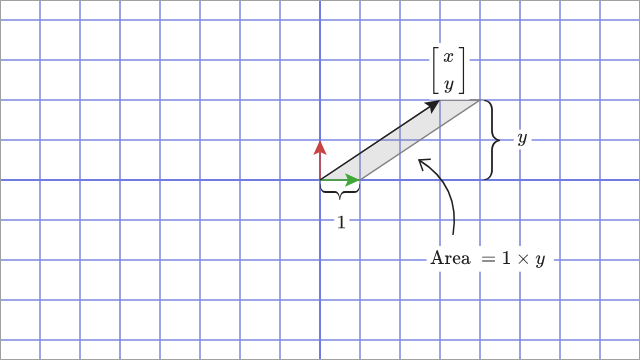
\includegraphics[width=0.7\textwidth]{./figs/det_exp_point.png}
    \caption{向量的另一种表示}
    \label{fig:det_exp_point}
\end{figure}

\begin{equation}
    \label{eq:example_lt_eq}
    \mat{2&-1\\0&1}\mat{x\\y}=\mat{4\\2}
\end{equation}

\begin{equation}
    \label{eq:2d_claw}
    x = \frac{Area}{det(A)} = \frac{det(\mat{4&-1\\2&1})}{det(\mat{2&-1\\0&1})}, y = \frac{Area}{det(A)} = \frac{det(\mat{2&4\\0&2})}{det(\mat{2&-1\\0&1})}
\end{equation}

\subsubsection{变基}

变基最朴素的理解是用一组新的基底来描述同一个向量(将向量视为标量与坐标系基的乘积)。如下公式~\ref{eq:change_basis_vector}所示,对于旧基 $\mat{1&0\\0&1}$ 新的基  $\mat{2&1\\-1&1}$(基于旧基描述),希望将新的基描述的$\mat{-1\\2}$使用旧基描述。

\begin{equation}
    \label{eq:change_basis_vector}
    \mat{2&1\\-1&1}\mat{-1\\2} = -1\mat{2\\1}+2\mat{-1\\1} = \mat{-4\\1}
\end{equation}

从几何上$\mat{2&1\\-1&1}$,将旧基的网格转为新基的网格;数值上将相同的向量使用旧基描述。

当我们将向量变换(新基$A$描述的向量,记为$\vec{v}$,旧基描述的变换(矩阵),记为$M$)考虑进来,按照前面的逻辑,需要做三步:1.将向量使用旧基表示 —— $A\vec{v}$;2.应用变换 —— $MA\vec{v}$;3.将变换后的向量(此时向量使用旧基描述)转为使用新基描述  —— $A^{-1}MA\vec{v}$。例如,对于逆时针旋转90°的变换($\mat{0&-1\\1&0}$):

\begin{enumerate}
    \item $\mat{2&-1\\1&1}\vec{v}$
    \item $\mat{0&-1\\1&0}\mat{2&-1\\1&1}\vec{v}$
    \item $\mat{2&-1\\1&1}^{-1}\mat{0&-1\\1&0}\mat{2&-1\\1&1}\vec{v}$
\end{enumerate}

表达式$A^{-1}MA$即是矩阵变基的公式

\subsubsection{特征值与特征向量}

\begin{figure}[hb]
    \centering
    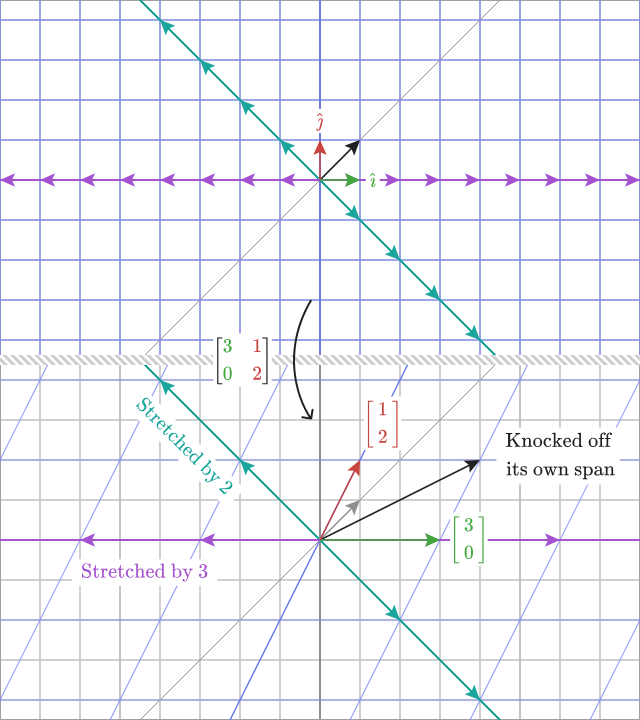
\includegraphics[width=0.7\textwidth]{./figs/eigenvec_remain_stay.png}
    \caption{特征向量在变换后方向不变}
    \label{fig:eigenvec_remain_stay}
\end{figure}

图~\ref{fig:eigenvec_remain_stay}最直观的展示了特征值与特征向量的几何含义:特征向量是哪些经过线性变换方向不改变的向量,只是被拉伸或者压缩一定的倍数,这个倍数就是特征值。

这是线性代数中经常出现的一种模式:对于任何由矩阵描述的线性变换,都可以通过读取矩阵的列作为基向量的落脚点来理解它在做什么。但是,要想了解变换的实际作用,最好的办法往往是找到特征向量和特征值,而不是依赖于特定的坐标系。

对于特征向量求解公式$A\vec{v}=\lambda\vec{v}$($A$描述线性变换,$\vec{v}$是特征向量,$\lambda$是特征值)的解释:等号的左侧是矩阵向量乘法,而等式右侧是标量乘法,因此需要将$\lambda$乘以单位矩阵$I$(对角线为1),此时公式可以被写为$A\vec{v}=(\lambda I)\vec{v}$,整理后得$(A-\lambda I)\vec{v} = \vec{0}$。由此当$\vec{v} \neq 0$时,我们寻找的$\lambda$其实是使$det(A-\lambda I) = 0$的$\lambda$

\textbf{对角矩阵}:考虑当基刚好是特征向量的情况,只要矩阵的对角线以外的地方都是零,它就被称为 "对角矩阵",所有的基向量都是特征向量,矩阵的对角线上的值就是相应的特征值。

\textbf{对角化}:如果变换有很多特征向量,足以选择一组横跨整个空间的特征向量,那么就可以改变坐标系,让这些特征向量成为基向量。参照变基中的公式,$A^{-1}MA$此时$A$为被选为基的特征向量(如对于特征向量$a_1,a_2$有$A=\mat{a_1^T&a_2^t}$),$M$为原始的变换

\section{Jacobian行列式与重积分}

Jacobian矩阵,如公式~\ref{eq:jacobianmatrix}所示,是一个$m\times n$矩阵,
其中$m$是方程个数,$n$是未知数个数。

\begin{equation}
    \label{eq:jacobianmatrix}
    J = \begin{bmatrix}
        \frac{\partial f_1}{\partial x_1} & \cdots & \frac{\partial f_1}{\partial x_n} \\
        \vdots  & \ddots & \vdots \\
        \frac{\partial f_m}{\partial x_1} & \cdots & \frac{\partial f_m}{\partial x_n}
    \end{bmatrix}
\end{equation}

\newpage

\bibliography{ref}
\bibliographystyle{unsrt}

\end{document}